
\section{GPGPU}

\subsection{A closer look at GPGPU\cite{Hu:2016:CLG:2891449.2873053}}

This paper introduces a formal model trying to generalize the computational model of GPUs.
It refers to \cite{nickolls2010gpu} as introducing a new computing era, called GPGPU.
There are many attempts of describing the internal mechanisms of GPU operation.
Some are focused on a graphics perspective, some others on general purpose.
New generation devices are surpassing this models and \cite{Hu:2016:CLG:2891449.2873053} tries to develop a broader model.
The task is difficult since most reports are either too simple or black-box descriptions \cite{Hu:2016:CLG:2891449.2873053}.
White papers focus on capabilities, programming guides on code syntax.
Some micro-architecture descriptions are too focused on a detail, ignoring the rest.

A hierarchical descriptive model for GPGPU is proposed in \cite{Hu:2016:CLG:2891449.2873053}.
It combines the ideas of the OpenCL and multi-BSP models (\textbf{TODO}).
A Processing Element of a higher level in the hierarchy sees lower-level Processing Elements as atomic.
The CUDA architecture is then described within this model as a two-level structure with nested components.
The architecture details are not public and won't probably ever be [Voicu 2010].
Thus the description has to be based on official patents and research papers.

\subsubsection{CUDA}
The GPU is the atomic element forming the second level of the hierarchy.
The first level is composed of the GigaThread Engine, CUDA Work Distributor, Data Transfer Engine, SM array, and local/global memory.
Each SM is broken into components of the 0th level.
These are the Thread controller, Warp scheduler, LSU, local/shared registers and ALU arrays.

Analogous components of different levels have different behaviours.
For example, the Processing Elements which are the ALU arrays (0th level) and SM array in (first level).
Each SM works asynchronously, whereas groups of ALUs have to work synchronously under a common program counter.
Other analogous components at different levels are LSU vs DTE arrays, local/shared registers vs local/global memory,
Task Buffers (program/block counters vs reference counter), Warp scheduler vs CWD, and Thread Controller vs GTE.

The principle behind the GPGPU advantages is dedicating more transistors to arithmetic logics and less to control.
That is why in CUDA a program counter is shared among 32 threads in a ``warp''.

All [\textbf{TODO:} Unified Memory] kernel input and output memory resides on device memory.
ALUs work on local/shared registers.
LSU array operations moving data in and out of these 2 memories are sped up through L2/L1 cache.
L2 cache is already on chip but outside the SMs, where L1 cache resides.

\subsubsection{Future Trends}

The current hierarchy consists of 2 levels, but this is not intrinsic to the model.
We could expect to see hierarchies with more levels or tasks of different levels being launched on the same hardware level.
Recursive kernel invocation and maybe the DGX-1 with faster interconnection between GPUs point in this direction.

We could also expect GPUs to part away from this Von Neumann hierarchical model and go in the way of neuromorphic chips.
These neuromorphic chips have ALUs and memory mixed, which allows simultaneous execution of different dataflows.

The hierarchical cache system reflects the convergence trend between CPU and GPU.
GPGPU is basically a hierarchical system of moving data to computing.
It could make sense to develop a system where computing is moved to data.

\subsection{The GPU computing era \cite{nickolls2010gpu}}

The GigaThread work scheduler balances work among SMs.
The SMs scheduler executes concurrent threads to help reduce the effect of long latency loads from DRAM memory.
DRAM memory in GPU and host CPU memory were linked with PCIe up to Pascal.


% \begin{figure}[h]%
%  	\begin{center}%
%  		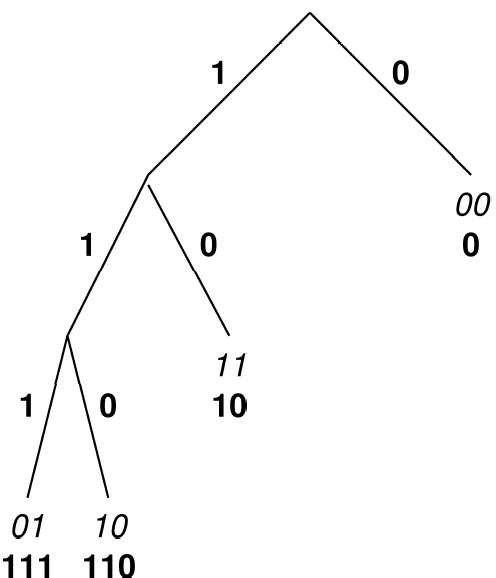
\includegraphics[scale=0.1]{figure1.png}%
%  		\caption{Baum}\label{fig:baum}%
%  	\end{center}%
% \end{figure}
%
% \begin{table}[h]%
%  	\begin{center}%
% 		\caption{Beispieltabelle}\label{tab:example}%
% 	 	\begin{tabular}{c|c}%
%  			Spalte1 & Spalte2\\
%  			\hline
%  			0 & 1\\
%  		\end{tabular}%
%  	\end{center}%
% \end{table}

% can use a bibliography generated by BibTeX as a .bbl file
% standard IEEE bibliography style from:
% http://www.ctan.org/tex-archive/macros/latex/contrib/supported/IEEEtran/bibtex
\bibliographystyle{IEEEtran}
% argument is your BibTeX string definitions and bibliography database(s)
\bibliography{IEEEabrv,references}
